% #####################################################################
% #####################################################################
% ##                                                                 ##
% ##                             Lizenz:                             ##
% ##                         CC BY-NC-SA 3.0                         ##
% ##      http://creativecommons.org/licenses/by-nc-sa/3.0/de/       ##
% ##                                                                 ##
% #####################################################################
% ##   Diese Datei kann beliebig verändert werden, solange darauf    ##
% ##     hingewiesen wird, dass dieses Dokument ursprünglich von     ##
% ##                                                                 ##
% ##                        www.ei-studium.de                        ##
% ##                                                                 ##
% ##                             stammt.                             ##
% ## Dies gilt insbesondere auch für alle daraus erstellten Dateien. ##
% ##    Des Weiteren muss die Weitergabe dieser Dateien unter der    ##
% ##                    gleichen Lizenz erfolgen.                    ##
% #####################################################################
% #####################################################################
\documentclass[a4paper,twocolumn,10pt]{article}
\usepackage[utf8]{inputenc}
\usepackage[ngerman]{babel}
\usepackage[top=2.0cm,bottom=1.5cm,left=1.0cm,right=1.0cm]{geometry}
\usepackage{enumitem}
\usepackage{graphicx}
\usepackage{amsfonts}
\usepackage{amsmath}
\usepackage{sectsty}
\usepackage{colortbl}
\usepackage{cancel}
\usepackage{listings}
\usepackage{color}
\usepackage{amsmath}
\usepackage{trfsigns}
\usepackage{epstopdf}
\usepackage{amssymb}
\usepackage{pdfpages}
\usepackage{fancyhdr}

\setlist{itemsep=.01mm}
\setenumerate{label=\emph{\arabic*})}
\setlength{\columnsep}{1cm}
\parindent 0mm

\partfont{\Large}
\sectionfont{\large \sc\bf}
\subsectionfont{\normalsize}
\subsubsectionfont{\small\textit}

\pagestyle{fancy}
\lhead[\leftmark]{Formelsammlung Elektrische Energietechnik}
\chead[\leftmark]{www.ei-studium.de}
\rhead[\leftmark]{Erstelldatum: \today}
\lfoot[\leftmark]{Keine Garantie auf Vollständigkeit und Richtigkeit!}
\cfoot[\leftmark]{}
\rfoot[\leftmark]{\thepage}
\renewcommand{\headrulewidth}{0.5pt}
\renewcommand{\footrulewidth}{0.5pt}

\newcommand{\sollsein}{\stackrel{!}{=}}

\begin{document}
\section{Wechselstromsystem}

\subsection{Effektivwert}
\begin{equation*}
\begin{split}
U_{\text{eff}}&=U=\sqrt{\frac{1}{T}\int\limits_Tu^2(\tau)d\tau}\\
U&=\frac{\hat{u}}{\sqrt{2}}\text{ für sinusförmige Größen}
\end{split}
\end{equation*}

\subsection{Phasenverschiebungswinkel}
\begin{equation*}
\varphi=\varphi_{ui}=\varphi_u-\varphi_i
\end{equation*}

\subsection{Elektrische Leistung}
Komplexe Leistung
\begin{equation*}
\underline{S}=\underline{U}\cdot\underline{I}^*=\frac{1}{2}\underline{\hat{u}}\cdot\underline{\hat{i}}^*=P+jQ
\end{equation*}
Komplexe Wechselleistung
\begin{equation*}
\underline{\tilde{S}}=\underline{U}\cdot\underline{I}=\frac{1}{2}\underline{\hat{u}}\cdot\underline{\hat{i}}
\end{equation*}
Momentanwert der Wechselleistung
\begin{equation*}
\tilde{p}(t)=Re\{\tilde{\underline{S}}\cdot e^{j2\omega t}\}
\end{equation*}
Leistungsfaktor
\begin{equation*}
\lambda=\frac{|P|}{S}=|\cos(\varphi)|
\end{equation*}
Wirkfaktor
\begin{equation*}
\cos(\varphi)=\frac{P_W}{S}
\end{equation*}
Blindfaktor
\begin{equation*}
\sin(\varphi)=\frac{Q}{S}
\end{equation*}

\subsection{Drehstromsystem}

\subsubsection{Symmetrisches Drehstromsystem}
\begin{equation*}
\begin{split}
U_1&=U_2=U_3\\
U_{12}&=U_{21}=U_{23}=U_{32}=U_{31}=U_{13}\\
U_{12}&=\sqrt{3}\cdot U_1\\
\underline{U}_1+\underline{U}_2+\underline{U}_3&=0\\
\underline{U}_{12}+\underline{U}_{23}+\underline{U}_{31}&=0
\end{split}
\end{equation*}

\subsubsection{Drehoperatoren}
\begin{equation*}
\begin{split}
\underline{a}&=e^{j\frac{2\pi}{3}}\\
\underline{U}_2&=\underline{a}^2\cdot\underline{U}_1\\
\underline{U}_3&=\underline{a}\cdot\underline{U}_1\\
1+\underline{a}+\underline{a}^2&=0
\end{split}
\end{equation*}

\subsubsection{Leistung}
Komplexe Leistung
\begin{equation*}
\begin{split}
\underline{S}&=\underline{U}_1\cdot\underline{I}_1^*+\underline{U}_2\cdot\underline{I}_2^*+\underline{U}_3\cdot\underline{I}_3^*\\
\underline{S}&=3\underline{U}_1\cdot\underline{I}_1^*\text{ falls symmetrisch}
\end{split}
\end{equation*}
Komplexe Wechselleistung
\begin{equation*}
\begin{split}
\underline{\tilde{S}}&=\underline{U}_1\cdot\underline{I}_1+\underline{U}_2\cdot\underline{I}_2+\underline{U}_3\cdot\underline{I}_3\\
\underline{\tilde{S}}&=0
\end{split}
\end{equation*}

\subsubsection{Sternschaltung}
\begin{center}
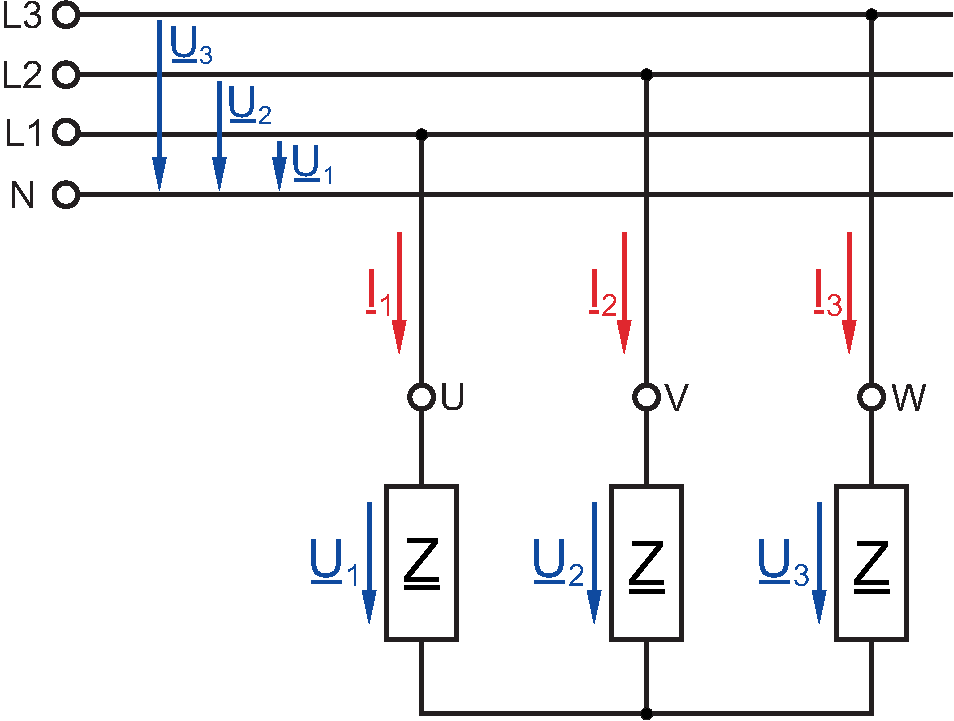
\includegraphics[width=0.8\columnwidth]{Grafiken/Sternschaltung}
\end{center}

\subsubsection{Dreieckschaltung}
\begin{center}
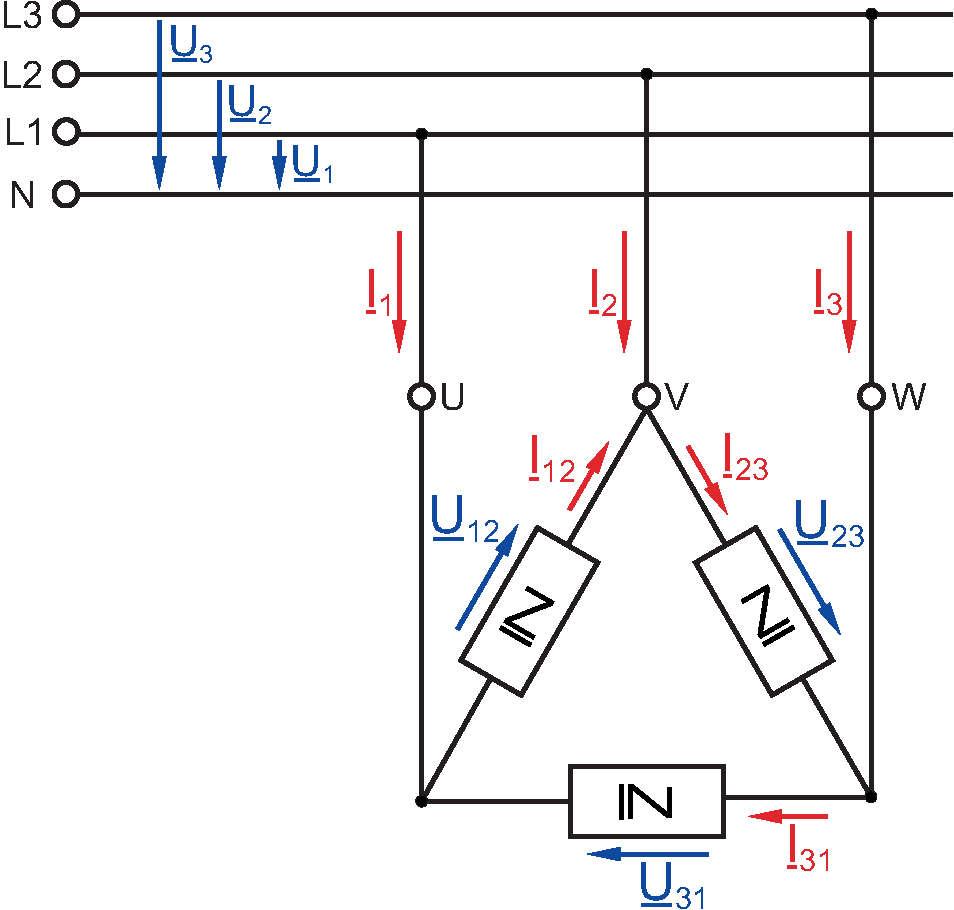
\includegraphics[width=0.8\columnwidth]{Grafiken/Dreieckschaltung}
\end{center}
\begin{equation*}
\begin{split}
\underline{I}_1&=\underline{I}_{12}-\underline{I}_{31}\\
\underline{I}_2&=\underline{I}_{23}-\underline{I}_{12}\\
\underline{I}_3&=\underline{I}_{31}-\underline{I}_{23}
\end{split}
\end{equation*}
Für ein symmetrisches System gilt außerdem:
\begin{equation*}
\begin{split}
\underline{I}&=|\underline{I}_1|=|\underline{I}_2|=|\underline{I}_3|\\
I_{\Delta}&=|\underline{I}_{12}|=|\underline{I}_{23}|=|\underline{I}_{31}|\\
I&=\sqrt{3}\cdot I_{\Delta}\\
U_{\Delta}&=|\underline{U}_{12}|=|\underline{U}_{23}|=|\underline{U}_{31}|
\end{split}
\end{equation*}

\begin{center}
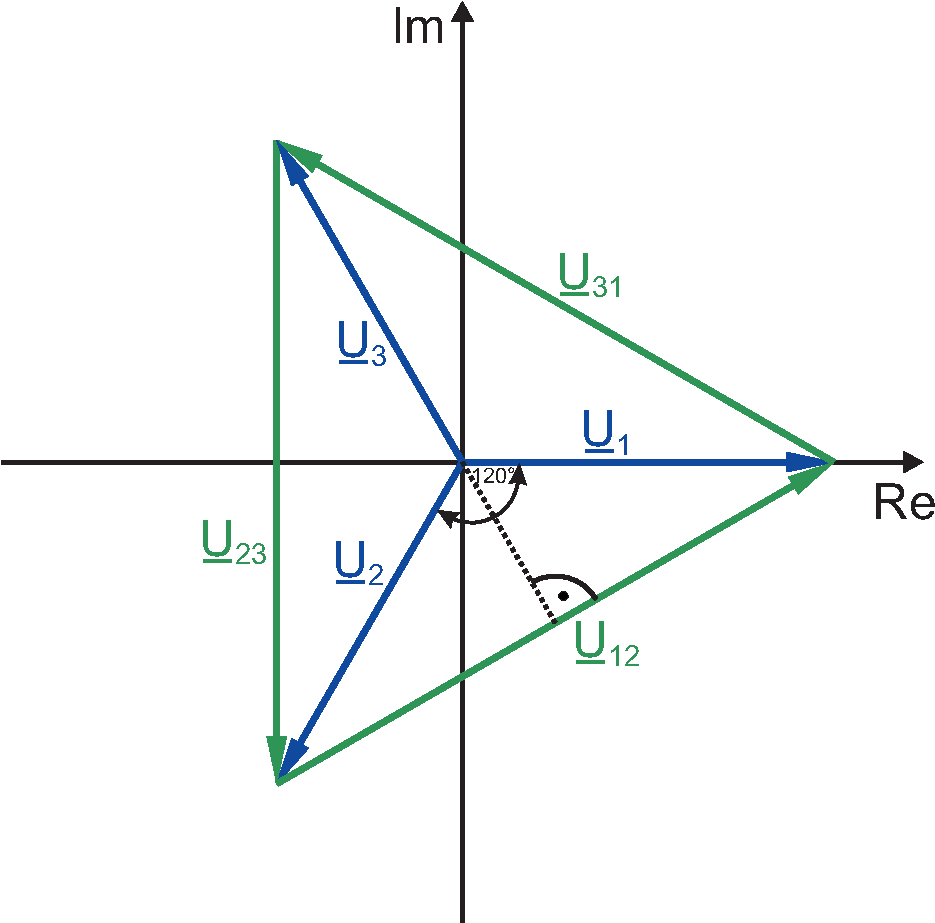
\includegraphics[width=0.8\columnwidth]{Grafiken/Drehstrom_Zeigerdiagramm}
\end{center}
\begin{center}
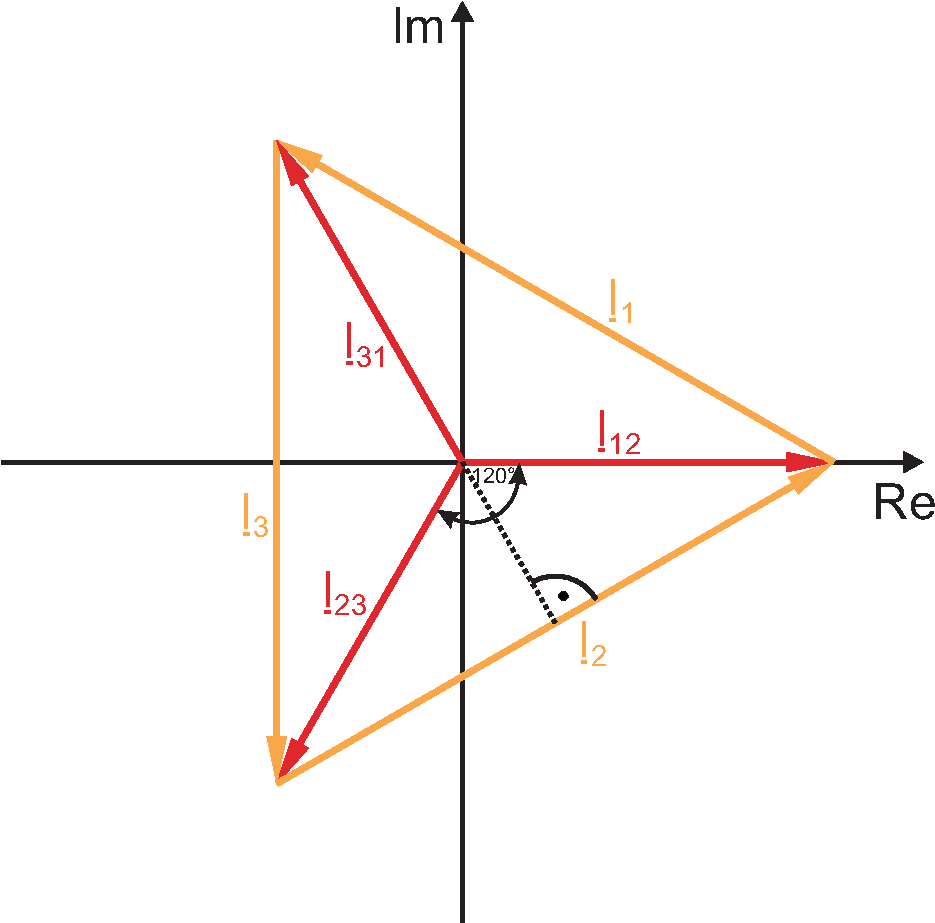
\includegraphics[width=0.8\columnwidth]{Grafiken/Drehstrom_Zeigerdiagramm_Strom}
\end{center}

\subsubsection{Kopplung der Leiter untereinander und zur Erde}
Die Kopplung kann wie folgt beschrieben werden:
\begin{equation*}
\begin{pmatrix}\underline{U}_1 \\ \underline{U}_2 \\ \underline{U}_3\end{pmatrix}=\begin{bmatrix}\underline{A} & \underline{B} & \underline{B} \\ \underline{B} & \underline{A} & \underline{B} \\ \underline{B} & \underline{B} & \underline{A}\end{bmatrix}\begin{pmatrix}\underline{I}_1 \\ \underline{I}_2 \\ \underline{I}_3\end{pmatrix}
\end{equation*}
$\underline{A}$: Eigenimpedanz längs des Leiters\\
$\underline{B}$: Koppelimpedanz zwischen den Leitern\\\\
Für den symmetrischen Fall vereinfacht sich dies zu:
\begin{equation*}
\begin{pmatrix}\underline{U}_1 \\ \underline{U}_2 \\ \underline{U}_3\end{pmatrix}=\underbrace{(\underline{A}-\underline{B})}_{\underline{Z}_b}\begin{pmatrix}\underline{I}_1 \\ \underline{I}_2 \\ \underline{I}_3\end{pmatrix}
\end{equation*}

\newpage
\section{Elektrische Maschinen}

\subsection{Transformator}

\subsubsection{Einphasiges ESB eines Transformators}
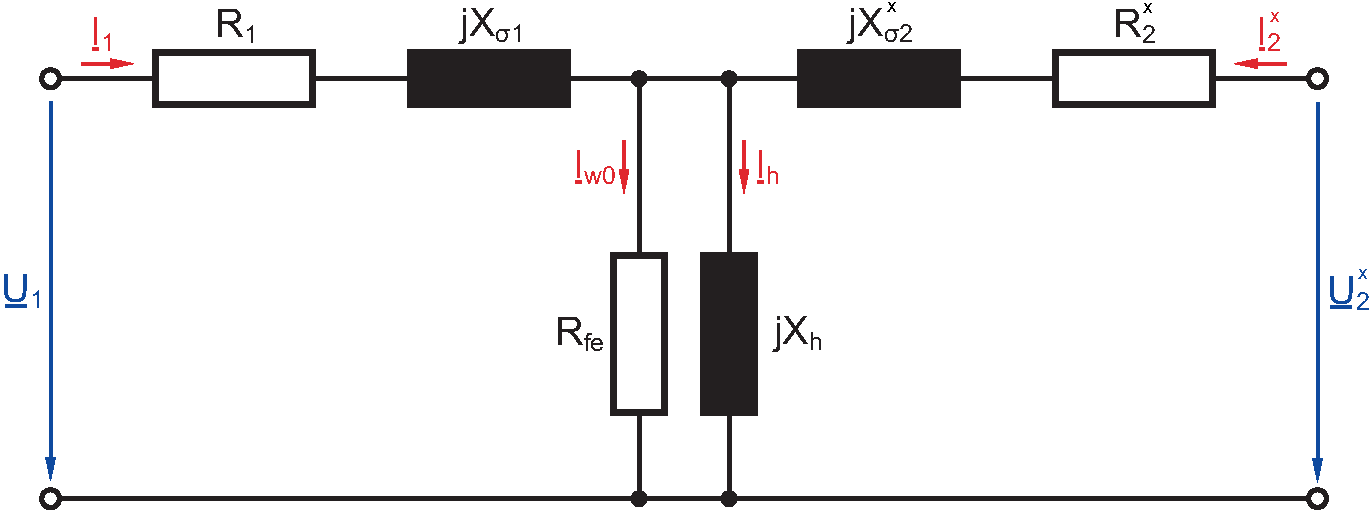
\includegraphics[width=0.9\columnwidth]{Grafiken/Trafo_ESB}\\\\
\begin{tabular}{ll}
$\text{ü}=\frac{w_1}{w_2}$ & Übersetzung\\
$\text{ü}=\frac{U_{r1T}}{U_{r2T}}\approx\frac{U_{n1}}{U_{n2}}$ & Übersetzung (bessere Definition)\\
$R_1$ & Ohmscher Widerstand der OS-Wicklung\\
$R_2^x=\text{ü}^2\cdot R_2$ & Ohmscher Widerstand der US-Wicklung\\
& auf OS-Seite bezogen\\
$X_{\sigma 1}$ & Streureaktanz der OS-Wicklung\\
$X_{\sigma2}^x=\text{ü}^2\cdot X_{\sigma 2}$ & Streureaktanz der US-Wicklung auf\\
&OS-Seite bezogen\\
$R_{Fe}$ & Eisenwiderstand\\
$X_h$ & Hauptreaktanz\\
$\underline{U}_1$ & Spannung auf der OS-Seite\\
$\underline{U}_2^x=\text{ü}\cdot\underline{U}_2$ & Spannung auf der US-Seite auf OS-Seite\\
& bezogen\\
$\underline{I}_1$ & Strom auf der OS-Seite\\
$\underline{I}_2^x=\frac{\underline{I}_2}{\text{ü}}$ & Strom auf der US-Seite auf OS-Seite\\
& bezogen\\
$S_{rT}$ & Bemessungsleistung\\
$U_{r1T}$ & Außenleiter-Bemessungsspannung
\end{tabular}
\begin{equation*}
\begin{split}
S_{rT}&=\sqrt{3}\cdot U_{r1T}\cdot I_r\\
Z_k&=\frac{U_k}{I_r}=u_k\cdot\frac{U_{r1T}^2}{S_{rT}}
\end{split}
\end{equation*}

\subsubsection{Leerlauf}
Im Leerlauf ($\underline{I}_2^x=0$) können der Widerstand $R_1$ und die Streureaktanz $X_{\sigma 1}$ vernachlässigt werden.\\
Für den Leerlaufstrom ergibt sich dann:
\begin{equation*}
I_{10}=\sqrt{I_{m0}^2+I_{w0}^2}\;\;\;\text{ mit }\underline{I}_{m0}=\underline{I}_h=\frac{\underline{U}_1}{jX_h}
\end{equation*}

\subsubsection{Dauerkurzschluss}
\begin{center}
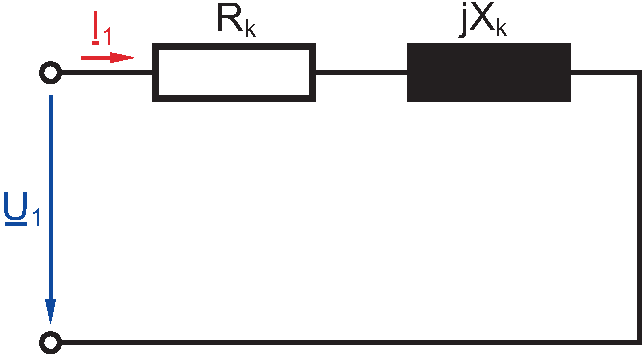
\includegraphics[width=0.6\columnwidth]{Grafiken/Trafo_KS_ESB}
\end{center}
\begin{equation*}
\begin{split}
u_k&=\frac{U_k}{U_r}=\frac{U_{kT}}{U_{r1T}}
\end{split}
\end{equation*}
\begin{tabular}{ll}
$U_k$: & Kurzschlussspannung ($=U_1$ bei Bemessungsstrom)\\
$U_{kT}$: & Kurzschlussspannung (Außenleiterspannung bei\\
& Bemessungsstrom)\\
$U_r$: & Bemessungsspannung (Leiter-Erde-Spannung)\\
$u_k$: & Relative Kurzschlussspannung
\end{tabular}


\subsubsection{Belastung mit Bemessungsstrom}
\begin{center}
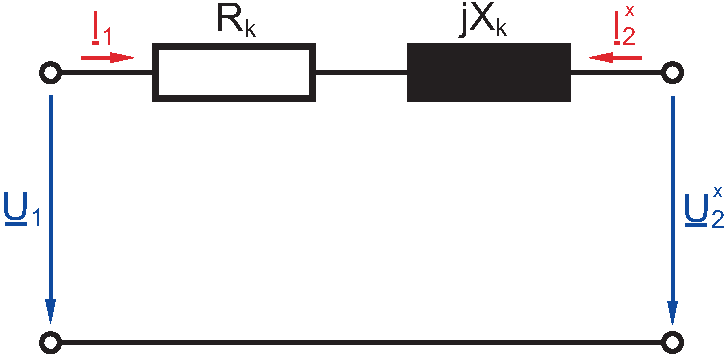
\includegraphics[width=0.6\columnwidth]{Grafiken/Trafo_BS_ESB}
\end{center}
\begin{equation*}
\begin{split}
R_k&=R_1+R_2^x\\
X_k&=X_{\sigma 1}+X_{\sigma 2}^x
\end{split}
\end{equation*}

\subsubsection{Drehstromtransformator}
Die Ersatzschaltbilder entsprechen den oben genannten, jedoch müssen die Spannungen durch $\sqrt{3}$ geteilt werden.

\subsection{Gleichstrommaschine (GMA)}
\begin{center}
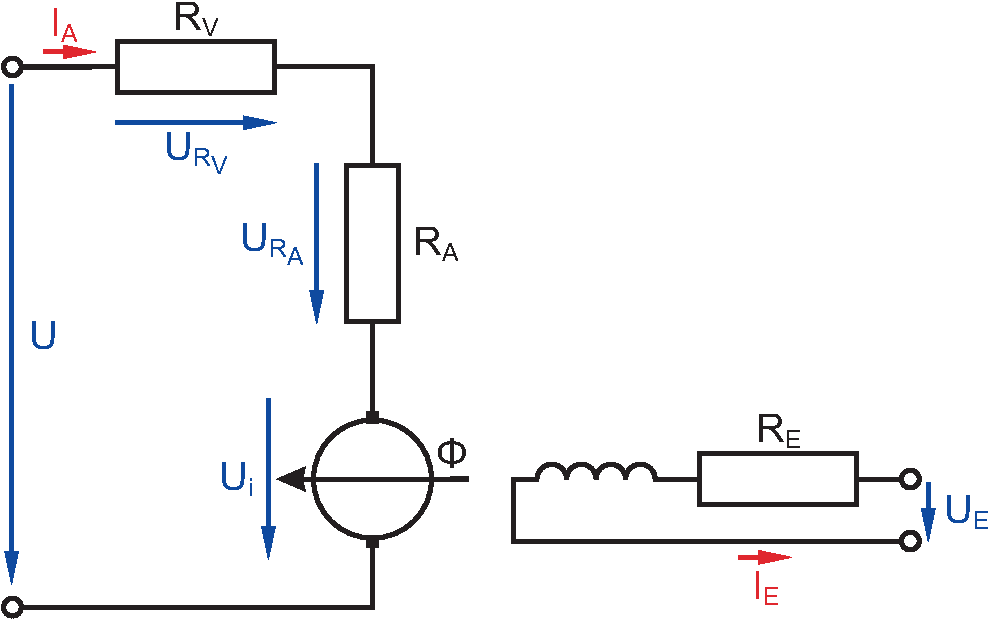
\includegraphics[width=0.95\columnwidth]{Grafiken/Gleichstrommaschine}
\end{center}
\begin{tabular}{ll}
$U$ & Klemmenspannung\\
$U_i$ & Im Anker induzierte Spannung\\
$I_A$ & Ankerstrom\\
$I_E$ & Erregerstrom\\
$R_A$ & Widerstand des Ankerkreises\\
$R_V$ & Vorwiderstand\\
$\Phi$ & Wirksamer magn. Fluss bei el. Erregung
\end{tabular}

\subsubsection{Grundgleichungen für den stationären Betrieb}
\begin{tabular}{ll}
$K_1,K_2$ & Maschinenkonstanten\\
$M$ & Drehmoment\\
$n$ & Drehzahl\\
$n_0$ & Leerlaufdrehzahl\\
$v$ & Geschwindigkeit\\
$r$ & Radius\\
$\Omega$ & Winkelgeschwindigkeit
\end{tabular}
\begin{equation*}
\begin{split}
R&=R_A+R_V\\
U&=U_i+R\cdot I_A=U_i+(R_A+R_V)I_A\\
U_i&=K_1\cdot\Phi\cdot n\\
M&=F\cdot r\\
M&=K_2\cdot\Phi\cdot I_A\\
K_1&=2\pi K_2\\
n&=\frac{1}{T}=\frac{v}{2\pi r}\\
\end{split}
\end{equation*}
\begin{equation*}
\begin{split}
n&=\underbrace{\frac{U}{K_1\cdot \Phi}}_{n_0}-\frac{R}{K_1\cdot K_2\cdot\Phi^2}\cdot M\\
n_0&=\frac{U}{K_1\cdot\Phi}=\frac{U\cdot n}{U_i}=\frac{U\cdot n}{U-R\cdot I_A}\\
\Omega&=2\pi n=\frac{v}{r}\\
P_{\text{mech}}&=M\cdot\Omega=F\cdot v=U_i\cdot I_A=P_{\text{el,A}}\\
P_{\text{el}}&=U\cdot I_A\\
P_R&=P_{\text{el}}-P_{\text{mech}}=I_A^2\cdot R
\end{split}
\end{equation*}

\subsubsection{GMA mit Fremderregung/Nebenschluss}
\begin{tabular}{ll}
$a$ & Beschleunigung\\
$m$ & Masse
\end{tabular}
\begin{equation*}
\begin{split}
M_{\text{min}}&=M+M_{a_\text{min}}=M+ F_{\text{min}}\cdot r=mr(g+a_{\text{min}})\\
M_{\text{max}}&=\frac{M\cdot I_{\text{max}}}{I_A}\\
n_0&=\frac{n_1-n_2\frac{M_1}{M_2}}{1-\frac{M_1}{M_2}}\\
R_{A0}&=R_{\text{V,max}}+R_A=\frac{U}{I_{\text{max}}}\\
\lambda&=\frac{M_{\text{max}}}{M_{\text{min}}}=\frac{I_{\text{an,max}}}{I_{\text{an}}}
\end{split}
\end{equation*}
\textbf{Berechnung der Stufenanzahl $z$ und der Vorwiderstände $R_{Vi}$:}
\begin{enumerate}
\item Berechne $z^*$:
\begin{equation*}
z^*=\lceil z\rceil=\left\lceil\frac{ln\left(\frac{R_{A0}}{R_A}\right)}{ln(\lambda)}\right\rceil
\end{equation*}
\item Berechne $\lambda^*$:
\begin{equation*}
\lambda^*=exp\left(\frac{ln\left(\frac{R_{A0}}{R_A}\right)}{z^*}\right)
\end{equation*}
\item Bestimme alle $R_{A0}$ bis $R_{Az^*}$:
\begin{equation*}
\begin{split}
\lambda^*&=\frac{M_{\text{max}}}{M_{\text{min}}}=\frac{I_{\text{max}}}{I_{\text{min}}}=\frac{R_{A0}}{R_{A1}}=\frac{R_{A1}}{R_{A2}}=...=\frac{R_{Az^*-1}}{R_{Az^*}}
\end{split}
\end{equation*}
\item Bestimme die in Reihe geschalteten Vorwiderstände:
\begin{equation*}
\begin{split}
R_A&=R_{Az^*}\\
R_{V1}&=R_{Az^*-1}-R_{Az^*}\\
&...\\
R_{Vz^*}&=R_{A0}-R_{A1}
\end{split}
\end{equation*}
\end{enumerate}

\subsubsection{Wirkungsgrad}
\begin{equation*}
\begin{split}
\eta_M&=\frac{P_{\text{mech}}}{P_{\text{el}}}=\frac{U_i}{U}\;\;\;\;\text{Motorbetrieb}\\
\eta_G&=\frac{P_{\text{el}}}{P_{\text{mech}}}=\frac{U}{U_i}\;\;\;\;\text{Generatorbetrieb}
\end{split}
\end{equation*}

\newpage
\subsection{Synchronmaschine (SMA)}
\begin{center}
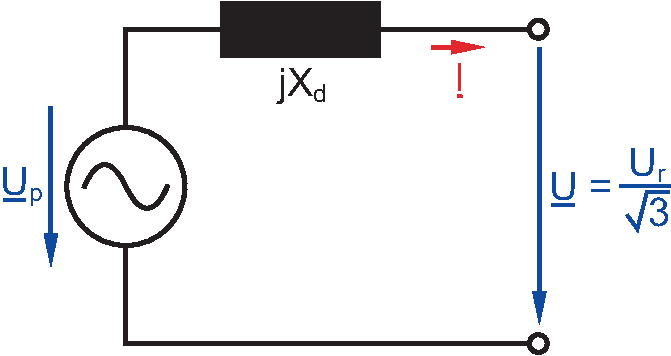
\includegraphics[width=0.7\columnwidth]{Grafiken/Synchronmaschine}
\end{center}
\begin{tabular}{ll}
$U$ & Klemmenspannung\\
$U_r$ & Bemessungsspannung (Außenleiterspannung)\\
$I$ & Strangstrom\\
$U_p$ & Polradspannung\\
$X_d$ & Synchrone Reaktanz\\
$S_r$ & Bemessungsscheinleistung (an Klemmen)\\
$P$ & Wirkleistung\\
$P_{VS}$ & Verlustleistung\\
$P_{VE}$ & Leistungsbedarf für die Erregung\\
$cos(\varphi)$ & Leistungsfaktor\\
$x_d$ & Bezogene synchrone Reaktanz\\
$Z_r$ & Bemessungsimpedanz\\
$n$ & Synchrone Drehzahl\\
$p$ & Anzahl der Polpaare\\
$\vartheta_M$ & Maschinenwinkel\\
$\omega$ & Winkelgeschwindigkeit der Spannung\\
$\Omega$ & Mechanische Winkelgeschwindigkeit
\end{tabular}
\begin{equation*}
\begin{split}
S_r&=\sqrt{3}\cdot U_r\cdot I_r\\
P&=S_r\cdot cos(\varphi)=3\cdot U\cdot I_w=\frac{3\cdot U\cdot U_P}{X_d}\cdot sin(\vartheta_M)\\
P_T&=P+P_{VS}+P_{VE}\\
x_d&=\frac{X_d}{Z_r}=\frac{\sqrt{3}\cdot X_d\cdot I_r}{U_r}\\
n&=\frac{f}{p}\\
\underline{U}&=\frac{\underline{U_r}}{\sqrt{3}}=\underline{U}_p-jX_d\underline{I}\\
cos(\vartheta_M)&=\frac{Re\{\underline{U}_p\}}{|\underline{U}_p|}\\
\omega&=p\cdot\Omega\\
I_w&=I_r\cdot cos(\varphi)\\
I_b&=I_r\cdot sin(\varphi)
\end{split}
\end{equation*}
\textbf{Übererregter Synchrongenerator:}
\begin{equation*}
\underline{I}=I_w-jI_b
\end{equation*}
$\Rightarrow$ wirkt im Netz wie eine Kapazität\\\\
\textbf{Untererregter Synchrongenerator:}
\begin{equation*}
\underline{I}=I_w+jI_b
\end{equation*}
$\Rightarrow$ wirkt im Netz wie eine Induktivität\\\\
\textbf{Phasenschieberbetrieb:}\\
Im Falle eines Phasenschieberbetriebs gilt: $I_w=0$

\subsection{Asynchronmaschine (AMA)}
\begin{center}
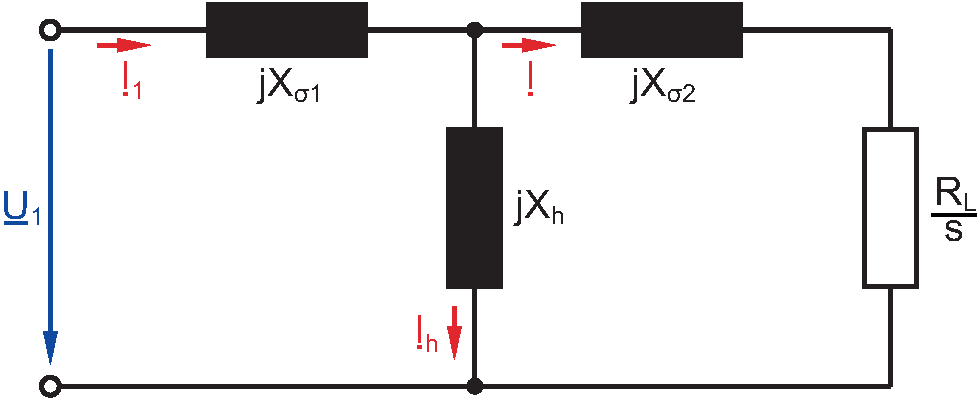
\includegraphics[width=0.9\columnwidth]{Grafiken/Asynchronmaschine}
\end{center}
Im Normalfall kann $jX_{\sigma1}$ vernachlässigt werden.\\
$\Rightarrow X_{\sigma 2}=X_{\sigma}$\\\\
\begin{tabular}{ll}
$U_r$ & Bemessungsspannung (Außenleiterspannung)\\
$U_1$ & Ständerspannung\\
$I_h$ & Magnetisierungsstrom\\
$X_{\sigma}$ & Streureaktanz\\
$X_h$ & Hauptreaktanz\\
$R_L$ & Läuferwiderstand\\
$f_0$ & Netzfrequenz\\
$n_0$ & Synchrone Drehzahl\\
$n_r$ & Drehzahl bei Nennbetrieb\\
$p$ & Polpaarzahl\\
$s$ & Schlupf\\
$s_r$ & Bemessungsschlupf\\
$s_k$ & Kippschlupf\\
$f_{SL}$ & Frequenz der im Läufer induzierten Spannung\\
$M_r$ & Bemessungsmoment\\
$M_{\text{an}}$ & Anlaufmoment\\
$M_k$ & Kippmoment\\
$P_r$ & Bemessungsleistung (= $P_{\text{ab}}$, falls Motor)\\
$S$ & Scheinleistung\\
$\eta$ & Wirkungsgrad
\end{tabular}\\\\\\
In der Regel gilt: $p\approx\frac{f_0}{n_r}$
\begin{equation*}
\begin{split}
n_0&=\frac{f_0}{p}\\
s&=\frac{n_0-n}{n_0};\;\;\;\;s_r=\frac{n_0-n_r}{n_0}\\
s_k&=\frac{R_L}{X_{\sigma}}\\
f_{SL}&=s\cdot f_0\\
P_r&=2\pi\cdot n_r\cdot M_r\\
M&=\frac{2M_K\cdot s_k\cdot s}{s_k^2+s^2}\;\;\;\;\text{(Kloss'sche Gleichung)}\\
M_k&=\frac{M_r\cdot\left(s_k^2+s_r^2\right)}{2\cdot s_k\cdot s_r}=\frac{3p\cdot U_1^2}{2\omega\cdot X_{\sigma}}=\frac{3p\cdot U_1^2}{8\pi^2\cdot L_{\sigma}\cdot f_1^2}\\
M_{\text{an}}&=\frac{2M_K\cdot s_k}{s_k^2+1};\;\;\;\;(n=0\rightarrow s=1)\\
\eta&=\frac{P_{\text{ab}}}{P_{\text{zu}}}=(1-s)\\
P_{\text{Verl}}&=P_{\text{zu}}-P_{\text{ab}}\\
\end{split}
\end{equation*}
Falls Motorbetrieb und $X_h=0$:
\begin{equation*}
\begin{split}
P_{\text{zu}}&=3I_r^2\cdot\frac{R_L}{s}=\sqrt{3}\cdot U_rI_rcos(\varphi)=S_{\text{zu}}\cdot cos(\varphi)\\
S_{\text{zu}}&=3\cdot I_r^2\cdot Z;\;\;\;Z^2=X_{\sigma}^2+\left(\frac{R_L}{s}\right)^2
\end{split}
\end{equation*}


\section{Übertragung elektrischer Energie}

\subsection{Vereinfachte Leitungsbetrachtung}
\begin{center}
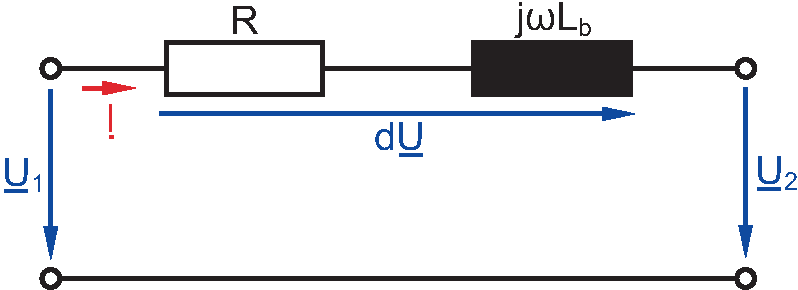
\includegraphics[width=0.8\columnwidth]{Grafiken/Uebertragungsleitung}
\end{center}
Vernachlässigung der Queradmittanzen bei hoher Belastung und kurzen Leitungen erlaubt (Freileitung: $l<$ 200 km; Kabel: $l<$ 100 km).\\
Für Hoch- und Mittelspannungsleitungen wird i.d.R. der ohmsche Längwiderstand $R$ vernachlässigt.
\begin{equation*}
\begin{split}
\omega L_b&=\omega L_b'\cdot l\\
R&=R'\cdot l\\
d\underline{U}&=\underline{U}_1-\underline{U}_2=\Delta U+j\delta U\\
\Delta U&=Re\{d\underline{U}\}\\
\delta U&=Im\{d\underline{U}\}\\
\underline{U}_2&=|\underline{U}_2|\cdot e^{j\varphi}\Rightarrow \underline{U}_1=|\underline{U}_1|\cdot e^{j(\varphi+\vartheta)}\\
tan(\vartheta)&=\frac{\delta U}{\Delta U+|\underline{U}_2|}\\
sin(\vartheta)&=\frac{\delta U}{|\underline{U}_1|}\\
P_1&=3\cdot|\underline{U}_1|\cdot |\underline{I}|\cdot cos(\varphi_{U_1I})=3\cdot |\underline{U}_1|\cdot I_w\\
P_2&=3\cdot|\underline{U}_2|\cdot |\underline{I}|\cdot cos(\varphi_{U_2I})=3\cdot |\underline{U}_2|\cdot I_w\\
Q_1&=3\cdot|\underline{U}_1|\cdot |\underline{I}|\cdot sin(\varphi_{U_1I})=3\cdot |\underline{U}_1|\cdot I_b\\
Q_2&=3\cdot|\underline{U}_2|\cdot |\underline{I}|\cdot sin(\varphi_{U_2I})=3\cdot |\underline{U}_2|\cdot I_b\\
P_{\text{Ltg}}&=P_1-P_2=3|\underline{I}|^2\cdot R\\
Q_{\text{Ltg}}&=Q_1-Q_2=3|\underline{I}|^2\cdot \omega L_b
\end{split}
\end{equation*}
$\underline{U}_2$ wird in die reelle Achse gelegt (Konvention).\\\\
Für ohmsch-induktive Verbraucher gilt:
\begin{equation*}
\begin{split}
d\underline{U}&=(I_w-jI_b)(R+j\omega L_b)\\
d\underline{U}&=\underbrace{R\cdot I_w+\omega L_b\cdot I_b}_{\Delta U}+j\underbrace{(\omega L_b\cdot I_w-R\cdot I_b)}_{\delta U}
\end{split}
\end{equation*}
Für ohmsch-kapazitive Verbraucher gilt:
\begin{equation*}
\begin{split}
d\underline{U}&=(I_w+jI_b)(R+j\omega L_b)\\
d\underline{U}&=\underbrace{R\cdot I_w-\omega L_b\cdot I_b}_{\Delta U}+j\underbrace{(\omega L_b\cdot I_w+R\cdot I_b)}_{\delta U}
\end{split}
\end{equation*}
Der Längsspannungsfall $\Delta U$ ist maßgebend für die Spannungshaltung längs der Leitung, während der Querspannungsfall $\delta U$ vorwiegend den Leitungswinkel $\vartheta$ und damit die Stabilität bestimmt.\\\\
\textbf{Konstruktion des Zeigerdiagramms:}\\
Gegeben seien $|\underline{U}_1|,|\underline{U}_2|,\vartheta$.
\begin{enumerate}
\item $\underline{U}_2$ einzeichnen (reelle Achse)
\item $\underline{U}_1$ einzeichnen
\item $d\underline{U}=\underline{U}_1-\underline{U}_2$ einzeichnen
\item $\Delta U$ und $\delta U$ einzeichnen mit $d\underline{U}=\Delta U+j\delta U$
\item $\underline{I}$ einzeichnen mit $|\underline{I}|=\frac{|d\underline{U}|}{\omega L_b}$ und $\underline{I}\perp d\underline{U}$ falls $R=0$
\item $I_w$ und $I_b$ einzeichnen mit $\underline{I}=I_w+jI_b$
\end{enumerate}

\subsection{Leitung als Vierpol}
\begin{center}
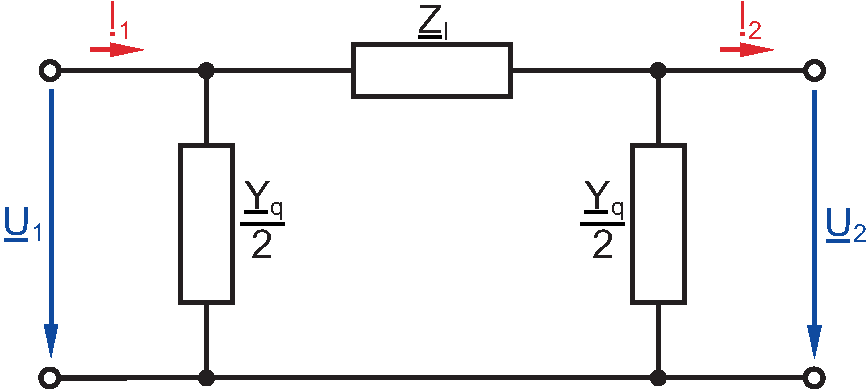
\includegraphics[width=0.8\columnwidth]{Grafiken/Vierpolleitung}
\end{center}
\begin{tabular}{ll}
$\underline{U}_1,\underline{U}_2$ & Sternspannungen\\
$Z_w$ & Betriebswellenwiderstand\\
$\beta$ & Phasenkonstante\\
$\vartheta$ & Leitungswinkel
\end{tabular}\\\\\\
Für lange Leitungen genügt die vereinfachte Leitungsbetrachtung nicht mehr, da der Wellencharakter der Leitung berücksichtigt werden muss.\\\\
Leitungsgleichungen für verlustlose Leitung:
\begin{equation*}
\begin{split}
\begin{bmatrix}\underline{U}_1 \\ \underline{I}_1\end{bmatrix}&=\begin{bmatrix}cos(\beta l) & jZ_wsin(\beta l) \\ \frac{j}{Z_w}sin(\beta l) & cos(\beta l)\end{bmatrix}\cdot\begin{bmatrix}\underline{U}_2 \\ \underline{I}_2\end{bmatrix}\\
Z_w&=\sqrt{\frac{\omega L_b'}{\omega C_b'}}\\
\beta&=\sqrt{\omega L_b'\cdot \omega C_b'}=\omega\sqrt{L_b'\cdot C_b'}\\
\vartheta&=\beta\cdot l\\
\underline{Z}_l&=jZ_w\cdot sin(\beta l)\\
\frac{\underline{Y}_q}{2}&=\frac{cos(\beta l)-1}{\underline{Z}_l}=\frac{cos(\beta l)-1}{jZ_w sin(\beta l)}
\end{split}
\end{equation*}
Speziell für kurze Leitungen (Freileitung: $l\leq$ 200 km bzw. Kabel: $l\leq 100$ km) gilt:
\begin{equation*}
\begin{split}
\underline{Z}_l&=j\omega L_b'l\\
\frac{\underline{Y}_q}{2}&=\frac{j\omega C_b'l}{2}
\end{split}
\end{equation*}

\subsection{Übertragung der natürlichen Leistung}
Natürliche Leistung ist die Leistung, die über eine Leitung übertragen werden kann, wenn sie mit dem Betriebswellenwiderstand $Z_w$ abgeschlossen ist.

\subsubsection{Übertragung der natürlichen Leistung $P_2=P_{\text{nat}}$}
\begin{equation*}
\begin{split}
\underline{I}_2&=\frac{\underline{U}_2}{Z_w}\\
\underline{U}_1&=\underline{U}_2e^{j\beta l}\\
\underline{I}_1&=\underline{I}_2\cdot e^{j\beta l}\\
\frac{\underline{U}_1}{\underline{I}_1}&=\frac{\underline{U}_2}{\underline{I}_2}=Z_w\\
P_{\text{nat}}&=3\cdot\frac{|\underline{U}_2|^2}{Z_w}=\frac{U_r^2}{Z_w}
\end{split}
\end{equation*}
Es wird somit nur Wirkleistung übertragen.

\subsubsection{Übertragung von $P_2<P_{\text{nat}}$}
$P_2<P_{\text{nat}}\Rightarrow Z_W\uparrow\;\;\;\;\Rightarrow L_b'\uparrow\text{ oder }C_b'\downarrow$\\\\
Ziel: $|\underline{U}_1|=|\underline{U}_2|,|\underline{I}_1|=|\underline{I}_2|$\\\\
\textbf{Längskompensation:} $L_b'\uparrow\;\;\;\;\Rightarrow\beta l\uparrow\;\;\;\;\Rightarrow\text{Stabilität }\downarrow$
\begin{center}
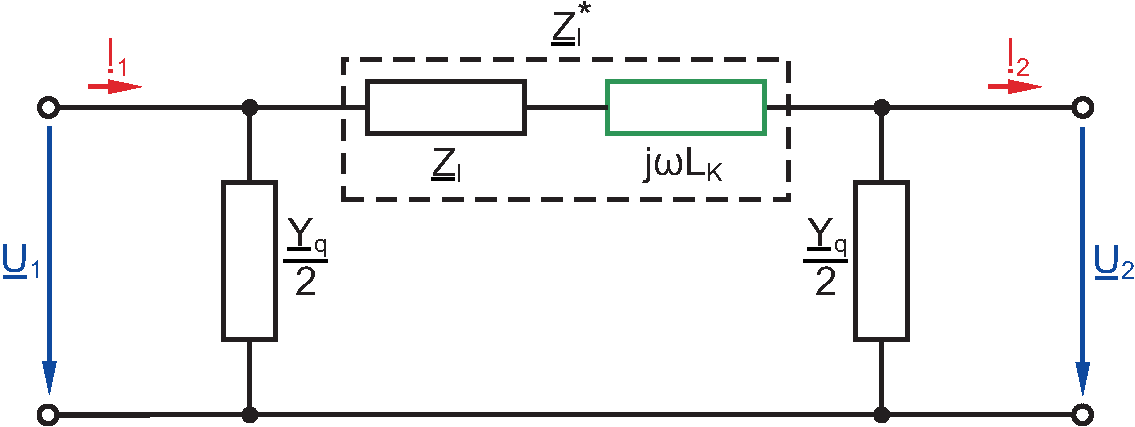
\includegraphics[width=0.98\columnwidth]{Grafiken/Laengskompensation_1}
\end{center}
\vspace{0.3cm}
\textbf{Querkompensation:} $C_b'\downarrow\;\;\;\;\Rightarrow\beta l\downarrow\;\;\;\;\Rightarrow\text{Stabilität }\uparrow$\\\\
\underline{Variante 1:}
\begin{center}
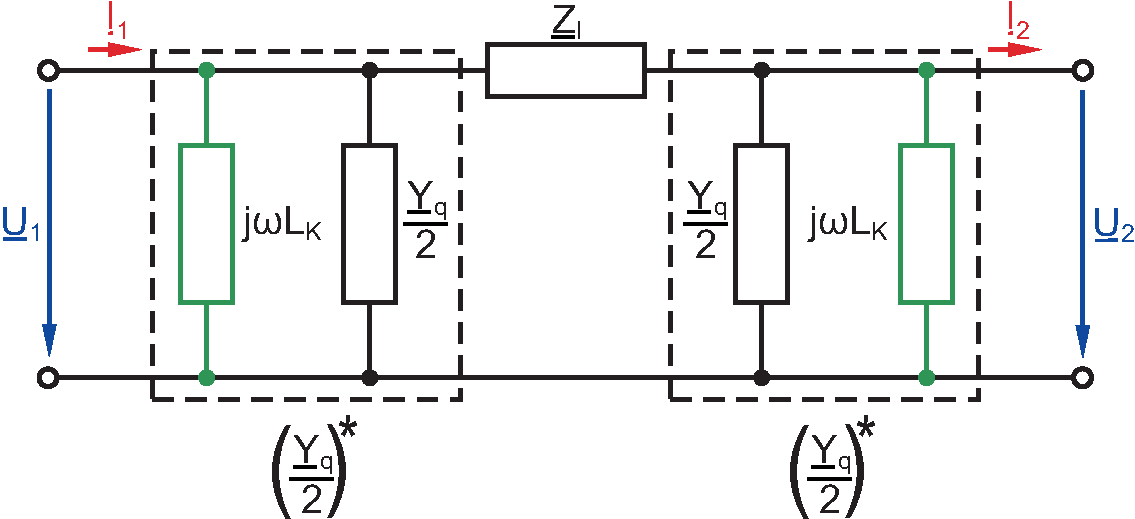
\includegraphics[width=0.98\columnwidth]{Grafiken/Querkompensation_1}
\end{center}
Vorgehensweise zum Berechnen von $L_K$:
\begin{enumerate}
\item Berechne
\begin{equation*}
Z_w^*=\frac{U_r^2}{P}
\end{equation*}
\item Berechne
\begin{equation*}
(\beta l)^*=arcsin\left(\frac{\underline{Z}_l}{jZ_w^*}\right)
\end{equation*}
\item Berechne
\begin{equation*}
\left(\frac{\underline{Y}_q}{2}\right)^*=\frac{cos\left((\beta l)^*\right)-1}{\underline{Z}_l}
\end{equation*}
\item Berechne $L_K$ mit
\begin{equation*}
\frac{1}{j\omega L_K}=\left(\frac{\underline{Y}_q}{2}\right)^*-\frac{\underline{Y}_q}{2}
\end{equation*}
\end{enumerate}
\underline{Variante 2:}
\begin{center}
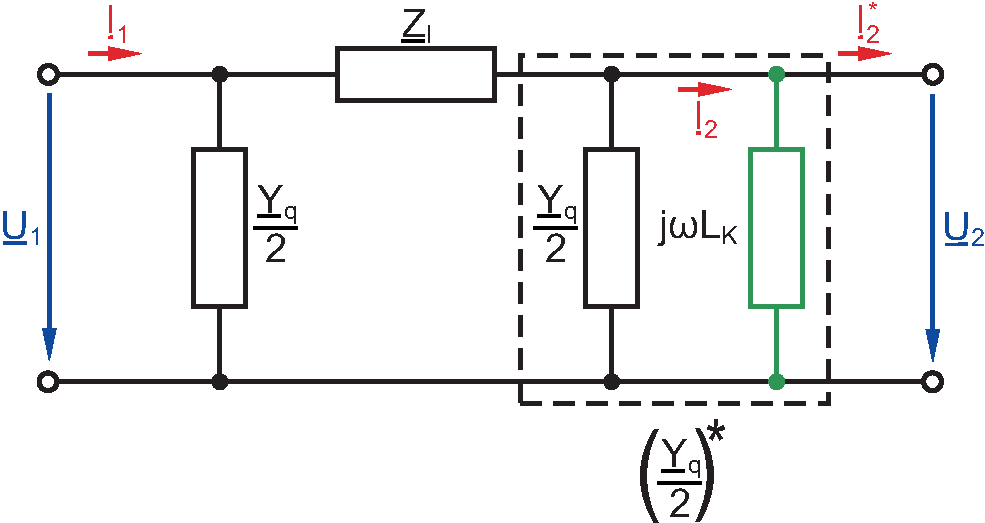
\includegraphics[width=0.85\columnwidth]{Grafiken/Querkompensation_12}
\end{center}

\subsubsection{Übertragung von $P_2>P_{\text{nat}}$}
$P_2>P_{\text{nat}}\Rightarrow Z_W\downarrow\;\;\;\;\Rightarrow L_b'\downarrow\text{ oder }C_b'\uparrow$\\\\
Ziel: $|\underline{U}_1|=|\underline{U}_2|,|\underline{I}_1|=|\underline{I}_2|$\\\\
\textbf{Längskompensation:} $L_b'\downarrow\;\;\;\;\Rightarrow\beta l\downarrow\;\;\;\;\Rightarrow\text{Stabilität }\uparrow$
\begin{center}
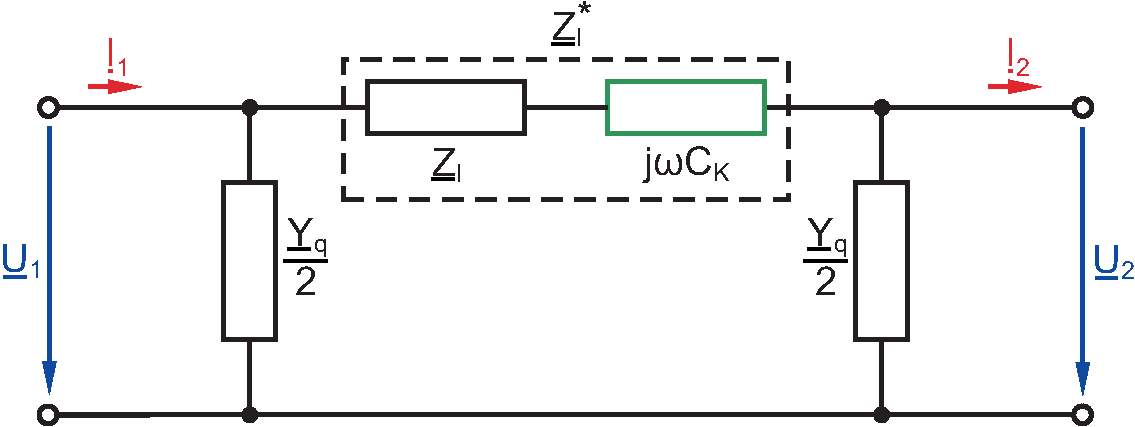
\includegraphics[width=0.98\columnwidth]{Grafiken/Laengskompensation_2}
\end{center}
\vspace{0.3cm}
\textbf{Querkompensation:} $C_b'\uparrow\;\;\;\;\Rightarrow\beta l\uparrow\;\;\;\;\Rightarrow\text{Stabilität }\downarrow$
\begin{center}
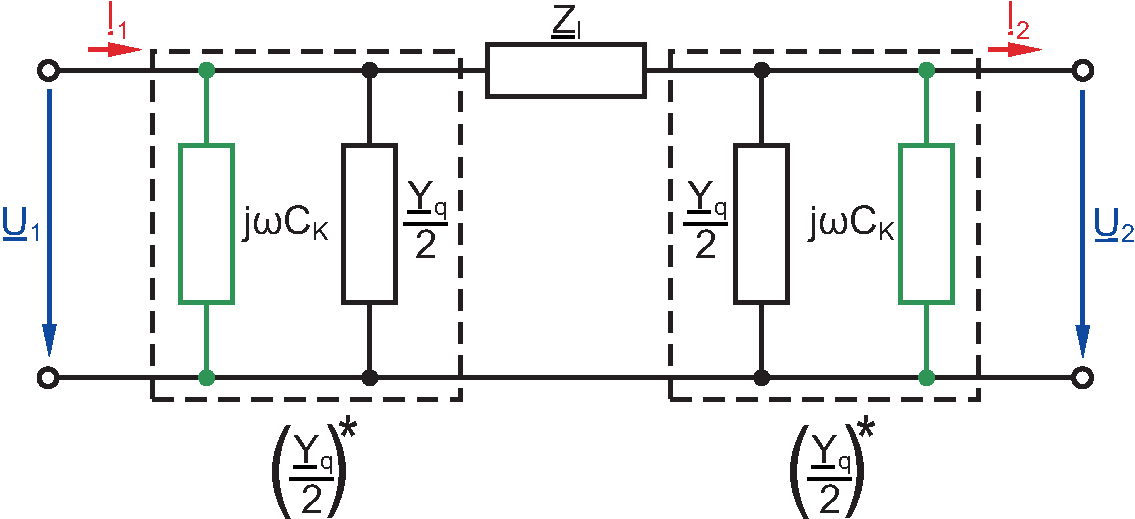
\includegraphics[width=0.98\columnwidth]{Grafiken/Querkompensation_2}
\end{center}
Vorgehensweise zum Berechnen von $C_K$:
\begin{enumerate}
\item Berechne
\begin{equation*}
Z_w^*=\frac{U_r^2}{P}
\end{equation*}
\item Berechne
\begin{equation*}
(\beta l)^*=arcsin\left(\frac{\underline{Z}_l}{jZ_w^*}\right)
\end{equation*}
\item Berechne
\begin{equation*}
\left(\frac{\underline{Y}_q}{2}\right)^*=\frac{cos\left((\beta l)^*\right)-1}{\underline{Z}_l}
\end{equation*}
\item Berechne $C_K$ mit
\begin{equation*}
j\omega C_K=\left(\frac{\underline{Y}_q}{2}\right)^*-\frac{\underline{Y}_q}{2}
\end{equation*}
\end{enumerate}
\newpage
\section{Hochspannungstechnik}

\subsection{Gasdurchschlag}
\begin{tabular}{ll}
$E_0$ & Innere elektrische Festigkeit von Luft\\
$E_{dh}$ & Durchschlaghöchstfeldstärke\\
$E_S$ & Spezifischer Spannungsbedarf einer Streamerentladung\\
$U^*$ & Spannungsbedarf der Streamerentladung\\
$U_i$ & TE-Einsetzspannung\\
$\eta$ & Homogenitätsgrad\\
$s$ & Elektrodenabstand
\end{tabular}
\begin{equation*}
\begin{split}
E_0&= 25\frac{kV}{cm}\;\;\;\;\text{(in Luft)}\\
E_S&=4,5\frac{kV}{cm}\;\;\;\;\text{(pos. Gleichspannung in Luft)}\\
E_S&=5-10\frac{kV}{cm}\;\;\;\;\text{(neg. Gleichspannung in Luft)}\\
U^*&=E_S\cdot s\\
U_i&=E_{dh}\cdot s\cdot \eta\\
\eta &=\frac{E_{\text{mittel}}}{E_{\text{max}}}=\frac{U}{E_{\text{max}}\cdot s}
\end{split}
\end{equation*}
\begin{tabular}{ll}
$\eta =1$ & Homogenes Feld\\
$\eta <1$ & Schwach inhomogenes Feld\\
$\eta <<1$ & Stark inhomogenes Feld
\end{tabular}

\subsubsection{Homogenes oder schwach inhomogenes Feld}
\begin{equation*}
\begin{split}
U^*&<U_i\\
U_d&=U_i=E_{dh}\cdot s\cdot\eta
\end{split}
\end{equation*}

\subsubsection{Stark inhomogenes Feld}
\begin{equation*}
\begin{split}
U^*&>U_i\\
U_d&=U^*=E_S\cdot s
\end{split}
\end{equation*}

\subsection{Lichtbogen}

\subsection{Versuchsaufbau}
\begin{center}
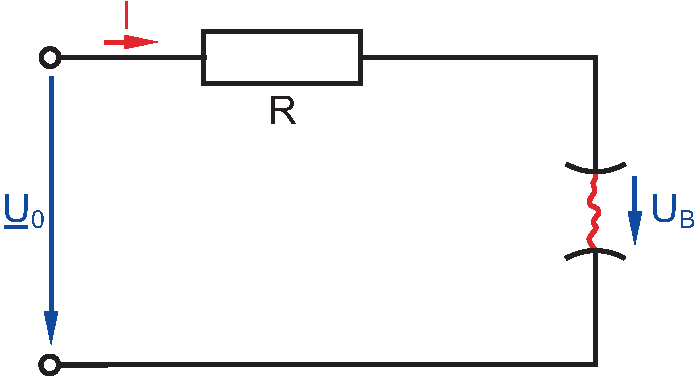
\includegraphics[width=0.7\columnwidth]{Grafiken/Lichtbogen_Stromkreis}
\end{center}
\begin{center}
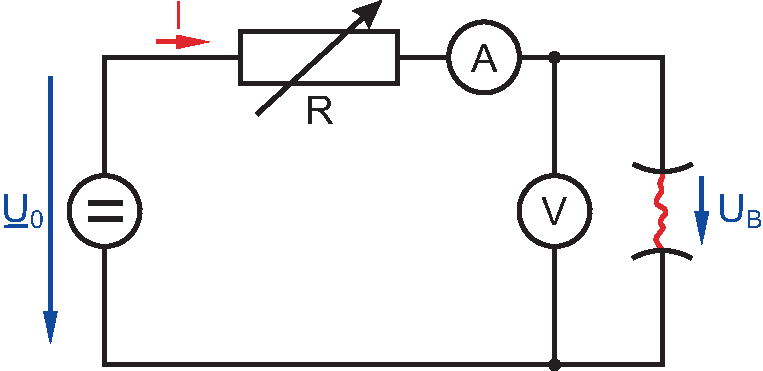
\includegraphics[width=0.7\columnwidth]{Grafiken/Lichtbogen_Stromkreis2}
\end{center}
\begin{tabular}{ll}
$U_B$ & Lichtbogenspannung\\
$R$ & Vorwiderstand\\
$U_0$ & Konstante Gleichspannung
\end{tabular}

\subsection{Kennlinie}
\begin{center}
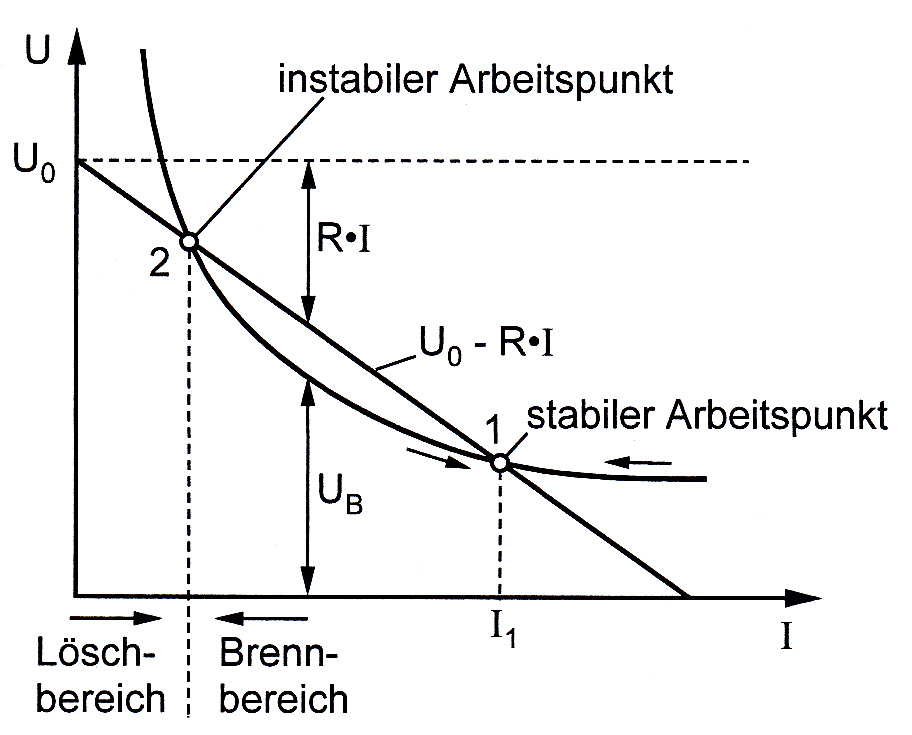
\includegraphics[width=0.98\columnwidth]{Grafiken/Lichtbogen}
\end{center}
\begin{equation*}
n\cdot U_B>U_{\text{Netz}}\;\;\;\;\text{(Löschbedingung)}\\
\end{equation*}
\begin{enumerate}[label=$\bullet$]
\item Instabiler AP:
\begin{enumerate}[label=-]
\item Auslenkung nach links:\\
$\rightarrow$ erhöhter Spannungsbedarf\\
(kann nicht aus Schaltung gedeckt werden)\\
$\rightarrow$ Lichtbogen erlischt
\item Auslenkung nach rechts:\\
$\rightarrow$ Strom wird größer\\
$\rightarrow$ Lichtbogen läuft in den stabilen AP
\end{enumerate}
\item Stabiler AP:
\begin{enumerate}[label=-]
\item Auslenkung nach rechts:\\
$\rightarrow$ Strom wird kleiner\\
$\rightarrow$ Lichtbogen läuft in den stabilen AP zurück
\end{enumerate}
\end{enumerate}

\subsubsection{Ayrton-Gleichung}
\begin{tabular}{ll}
$l$ & Lichtbogenlänge\\
$a,b,c,d$ & Materialabhängige Konstanten\\
$n$ & Anzahl der Teillichtbögen
\end{tabular}
\begin{equation*}
\begin{split}
n\cdot U_B&>U_{\text{max}}\;\;\;\;\text{(Löschbedingung)}\\
U_B&=a+b\cdot l+\frac{c+d\cdot l}{I}=U_0-R\cdot I\\
\Rightarrow l&=\frac{U_B-a-\frac{c}{I}}{b+\frac{d}{I}}\\
\Rightarrow I_{1,2}&=\frac{-(a+bl-U_0)\pm\sqrt{(a+bl-U_0)^2-4R(c+dl)}}{2R}
\end{split}
\end{equation*}\\\\
Für $R_{\text{max}}, U_{0_{\text{min}}}$ und $l_{\text{max}}$ muss die Diskriminante gleich Null gesetzt werden:
\begin{equation*}
(a+bl-U_0)^2-4R(c+dl)\sollsein 0
\end{equation*}
\begin{enumerate}[label=$\bullet$]
\item $R_{\text{max}}$:
\begin{equation*}
\Rightarrow R_{\text{max}}=\frac{(a+bl-U_0)^2}{4(c+dl)}
\end{equation*}
\item $U_{0_{\text{min}}}$:
\begin{equation*}
U_0^2+\underbrace{[-2(a+bl)]}_{B}U_0+\underbrace{[a^2+(bl)^2+2abl-4R(C+dl)]}_{C}=0
\end{equation*}
\begin{equation*}
\Rightarrow U_{0\text{min}_{1/2}}=\frac{-B\pm\sqrt{B^2-4C}}{2}
\end{equation*}
\item $l_{\text{max}}$:
\begin{equation*}
\underbrace{b^2}_{A}l^2+\underbrace{(2ab-2bU_0-4Rd)}_{B}l+\underbrace{(a^2-2aU_0+U_0^2-4Rc)}_{C}=0
\end{equation*}
\begin{equation*}
\Rightarrow l_{\text{max}_{1/2}}=\frac{-B\pm\sqrt{B^2-4AC}}{2A}
\end{equation*}
\end{enumerate}

\subsection{Löschung}
\begin{tabular}{ll}
$n$ & Anzahl der Teillichtbögen
\end{tabular}
\begin{equation*}
\begin{split}
n\cdot U_B&>U_{\text{max}}\;\;\;\;\text{(Löschbedingung)}\\
\end{split}
\end{equation*}
Bei einem Blechabstand von wenigen Millimetern gilt: $U_B\approx 20V$.
\\\\\\\\
Lizenz: CC BY-NC-SA 3.0\\
http://creativecommons.org/licenses/by-nc-sa/3.0/de/

\end{document}








